% Source for the figure of SuffixArray (sec. 15.5): the suffix array, the
% LCP array and the suffixes of banana, in rank order, with the range of
% the pattern an (shaded) that range() finds by two binary searches.
% Build: make figures (in ../build).
\documentclass[border=4pt]{standalone}
\usepackage[T1]{fontenc}
\usepackage{newpxtext,newpxmath}
\usepackage[varqu,varl,scaled=0.95]{zi4}
\usepackage{tikz}
% tikz-ads.tex: the TikZ styles shared by the figures of the memory of the
% manual, \input by each standalone figure: a cell of a vector (cell), the
% cell that an operation touches (touched), a free cell (free), a node of a
% linked structure (node), the labels of indices (index) and of variables
% (var), a pointer (ptr), and \cells and \indices to draw a row of cells.
\usetikzlibrary{arrows.meta,positioning,calc,fit,shapes.multipart}
\definecolor{adsTouched}{RGB}{214,196,236}
\definecolor{adsFree}{RGB}{236,236,236}
\tikzset{
  ads/.style={>={Stealth[length=2mm]},font=\small,
              every node/.append style={inner sep=0pt}},
  cell/.style={draw,minimum width=7mm,minimum height=7mm,
               font=\small\ttfamily,outer sep=0pt},
  touched/.style={cell,fill=adsTouched},
  free/.style={cell,fill=adsFree,text=black!45},
  node/.style={draw,rounded corners=1pt,minimum width=8mm,
               minimum height=6mm,font=\small\ttfamily},
  index/.style={font=\scriptsize\ttfamily,text=black!60},
  var/.style={font=\small\itshape},
  ptr/.style={->,thick}
}
% \cells{name}{x,y}{list}: a row of cells, the first at (x,y), named
% name-0, name-1, ...; each item is text/style, the style one of cell,
% touched and free (e.g., {a/cell,e/touched,/free})
\newcommand{\cells}[3]{%
  \foreach \v/\s [count=\i from 0] in {#3}
    \node[\s] (#1-\i) at ($(#2)+(\i*7mm,0)$) {\v};}
% \indices{name}{n}: the indices 0 .. n-1 under the cells of name
\newcommand{\indices}[2]{%
  \foreach \i in {0,...,\numexpr#2-1\relax}
    \node[index,below=1.2mm of #1-\i] {\i};}

\usetikzlibrary{decorations.pathreplacing}
\begin{document}
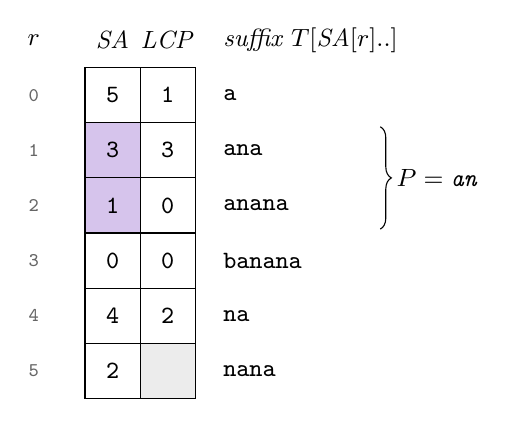
\begin{tikzpicture}[ads]
  \node[var] at (0,7mm) {$r$};
  \node[var] at (10mm,7mm) {$\mathit{SA}$};
  \node[var] at (17mm,7mm) {$\mathit{LCP}$};
  \node[var,anchor=west] at (24mm,7mm) {suffix $T[ \mathit{SA}[ r ] .. ]$};
  \foreach \r/\sa/\lcp/\suf/\st in {0/5/1/a/cell,1/3/3/ana/touched,
      2/1/0/anana/touched,3/0/0/banana/cell,4/4/2/na/cell,5/2//nana/cell} {
    \node[index] at (0,-\r*7mm) {\r};
    \node[\st] at (10mm,-\r*7mm) {\sa};
    \node[cell] at (17mm,-\r*7mm) {\lcp};
    \node[font=\small\ttfamily,anchor=west] at (24mm,-\r*7mm) {\suf};
  }
  \node[free] at (17mm,-35mm) {};
  \draw[decorate,decoration={brace,amplitude=4pt}]
    (44mm,-4mm) -- node[right=2mm,var] {$P = \texttt{an}$} (44mm,-17mm);
\end{tikzpicture}
\end{document}
